\section*{Supplementary Material}
\subsection*{Derivation of G(r,t)}

We first define an ensemble of k identical brownian bugs in a 2-dimension
space (the following can easily be generalized to d dimensions). The
bug number p is located at $\boldsymbol{x}_{p}=[x1,x2,...x_{k}]$.
At time $t$, the space is defined by (a) the number of browninan
bugs $k$ and (b) the vector of their locations $\boldsymbol{X}_{k}=[\boldsymbol{x}_{1},\boldsymbol{x}_{2},...\boldsymbol{x}_{k}]$.
This is also called the Fock space. The probability distribution over
the state space is given by the functions $\mathcal{P}_{k}(\boldsymbol{X}_{k},t)$
such that:

\begin{equation}
\mathcal{P}_{k}(\boldsymbol{X}_{k},t)d\boldsymbol{X}_{k}=\text{Pr}\{k\text{ bugs, with a bug in }d\boldsymbol{x}_{1},\text{a bug in }d\boldsymbol{x}_{2}\text{, etc.}\}
\end{equation}

As bugs are indistinguishable, we can exchange $\boldsymbol{x}_{p}$
and $\boldsymbol{x}_{q}$:

\begin{equation}
\mathcal{P}_{k}(\boldsymbol{x}_{1},\ldots,\boldsymbol{x}_{p},\ldots,\boldsymbol{x}_{q},\ldots,\boldsymbol{x}_{k},t)=\mathcal{P}_{k}(\boldsymbol{x}_{1},\ldots,\boldsymbol{x}_{q},\ldots,\boldsymbol{x}_{p},\ldots,\boldsymbol{x}_{k},t)
\end{equation}

The normalization is: 

\begin{equation}
\mathcal{P}_{0}(t)+\int\mathcal{P}_{1}(\boldsymbol{X}_{k},t)d\boldsymbol{x}_{1}+\int\int\mathcal{P}_{2}(\boldsymbol{X}_{k},t)d\boldsymbol{x}_{1}d\boldsymbol{x}_{2}+\ldots+\int_{R^{2k}}\mathcal{P}_{k}(\boldsymbol{X}_{k},t)d\boldsymbol{X}_{k}=1
\end{equation}

We define $b_{k}(\mathbf{x},t)=\int\mathcal{P}_{k}(\boldsymbol{x},\boldsymbol{X}_{k-1},t)d\boldsymbol{X}_{k-1}$,
the probability that there are $k$ bugs and bug number 1 is in $d\boldsymbol{x}$.\\

The density of points is defined as:

\begin{equation}
\rho(\boldsymbol{x},t)=\sum_{k=1}^{\infty}kb_{k}(\boldsymbol{x},t)=\sum_{k=1}^{\infty}k\int\mathcal{P}_{k}(\boldsymbol{x},\boldsymbol{X}_{k-1},t)d\boldsymbol{X}_{k-1}
\end{equation}

The pair correlation function is then:

\begin{equation}
G(\boldsymbol{x},\boldsymbol{y},t)=\sum_{k=2}^{\infty}k(k-1)\int\mathcal{P}_{k}(\boldsymbol{x},\boldsymbol{y},\boldsymbol{X}_{k-2},t)d\boldsymbol{X}_{k-2}-\rho(\boldsymbol{x},t)\rho(\boldsymbol{y},t)\label{eq:def_pairdens}
\end{equation}

We define $\eta(\boldsymbol{x},\boldsymbol{y},t)=\sum_{k=2}^{\infty}k(k-1)\int\mathcal{P}_{k}(\boldsymbol{x},\boldsymbol{y},\boldsymbol{X}_{k-2},t)d\boldsymbol{X}_{k-2}$
and the two particle distribution functions $c_{k}(\boldsymbol{x},\boldsymbol{y},t)=\int\mathcal{P}_{k}(\boldsymbol{x},\boldsymbol{y},\boldsymbol{X}_{k-2},t)d\boldsymbol{X}_{k-2}$.
Note that $\eta(\boldsymbol{x},\boldsymbol{y},t)=\sum_{k=2}^{\infty}k(k-1)c_{k}(\boldsymbol{x},\boldsymbol{y},t)$.

\vspace{2em}


\paragraph*{Diffusion and birth/death processes}

We now write the evolution of $\mathcal{P}_{k}(\boldsymbol{X}_{k},t)$:

\begin{subequations} 
\begin{align}
\frac{\partial\mathcal{P}_{k}}{\partial t} & =D\nabla_{k}^{2}\mathcal{P}_{k}\label{pk_diffusion}\\
 & -k(\lambda+\mu)\mathcal{P}_{k}\label{pk_same_state}\\
 & +(k+1)\mu\int\mathcal{P}_{k+1}(\boldsymbol{X}_{k},\boldsymbol{y},t)d\boldsymbol{y}\label{pk_death}\\
 & +\frac{\lambda}{k}\sum_{p=1}^{k}\sum_{q=1,q\neq p}^{k}\delta_{pq}\mathcal{P}_{k-1}(\boldsymbol{X}_{k|p,t})\label{pk_birth}
\end{align}
\end{subequations}

where $\nabla_{k}^{2}=\frac{\partial^{2}}{\partial_{x_{1}}^{2}}+\frac{\partial^{2}}{\partial_{y_{1}}^{2}}+\ldots+\frac{\partial^{2}}{\partial_{x_{k}}^{2}}+\frac{\partial^{2}}{\partial_{y_{k}}^{2}}$,
$\delta_{pq}=\delta(\boldsymbol{x}_{p}-\boldsymbol{x}_{q})$ and $\boldsymbol{X}_{k|p}=\boldsymbol{X}_{k}$
with $\boldsymbol{x}_{p}$ deleted. \\

Note that

\begin{align}
\mathcal{P}(\boldsymbol{X}_{k|p})\delta_{pq}d\boldsymbol{x}_{1}\ldots d\boldsymbol{x}_{k} & =\int\delta(\boldsymbol{x}_{p}-\boldsymbol{x}_{q})\mathcal{P}(\boldsymbol{x}_{1}\ldots\boldsymbol{x}_{q}\ldots\boldsymbol{x}_{p-1}\boldsymbol{x}_{p+1}\ldots\boldsymbol{x}_{k})d\boldsymbol{x}_{1}\ldots d\boldsymbol{x}_{q}\ldots d\boldsymbol{x}_{p}\ldots d\boldsymbol{x}_{k}\\
 & =?????\label{eq:missing_step}\\
\Leftrightarrow\int\mathcal{P}(\boldsymbol{X}_{k|p})\delta_{pq}d\boldsymbol{X}_{k} & =\int\mathcal{P}(\boldsymbol{X}_{k-1})d\boldsymbol{X}_{k-1}\label{delta_simplify}
\end{align}

Here, eq. \ref{pk_diffusion} is the diffusion part of the process,
eq. \ref{pk_same_state} corresponds to the case in which we leave
a state of $k$ particles because one of them dies or reproduces ,
eq. \ref{pk_death} represents the shit from a $k+1$ bug state to
a $k$ bug state due to the death of a particle and eq. \ref{pk_birth}
represents the production of a particle from a realization with $k-1$
bugs to $k$ bugs due to the reproduction of one particle.

Using the derivation of $\mathcal{P}_{k}(\boldsymbol{X}_{k},t)$ and
the definition of $c_{k}$, we have:

\begin{subequations} 
\begin{align}
\frac{\partial c_{k}}{\partial t}(\boldsymbol{x},\boldsymbol{y},t) & =D\int\nabla_{k}^{2}\mathcal{P}_{k}(\boldsymbol{x},\boldsymbol{y},\boldsymbol{X}_{k-2},t)d\boldsymbol{X}_{k-2}\label{ck_diffusion}\\
 & -k(\lambda+\mu)\int\mathcal{P}_{k}(\boldsymbol{x},\boldsymbol{y},\boldsymbol{X}_{k-2},t)d\boldsymbol{X}_{k-2}\label{ck_same_state}\\
 & +(k+1)\mu\int\mathcal{P}_{k+1}(\boldsymbol{x},\boldsymbol{y},\boldsymbol{X}_{k-2},\boldsymbol{z},t)d\boldsymbol{X}_{k-2}d\boldsymbol{z}\label{ck_death}\\
 & +\frac{\lambda}{k}\int\sum_{p=1}^{k}\sum_{q=1,q\neq p}^{k}\delta_{pq}\mathcal{P}_{k-1}(\boldsymbol{X}_{k|p,t})\label{ck_birth}
\end{align}
\end{subequations}

We will treat one term after the other. \\


\subsubsection*{Diffusion term (\ref{ck_diffusion})}

:

\begin{subequations} 
\begin{align}
D\int\nabla_{k}^{2}\mathcal{P}_{k}(\boldsymbol{x},\boldsymbol{y},\boldsymbol{X}_{k-2},t)d\boldsymbol{X}_{k-2} & =D\nabla_{k}^{2}\int\mathcal{P}_{k}(\boldsymbol{x},\boldsymbol{y},\boldsymbol{X}_{k-2},t)d\boldsymbol{X}_{k-2}\\
 & =D\nabla_{2}^{2}\int\mathcal{P}_{k}(\boldsymbol{x},\boldsymbol{y},\boldsymbol{X}_{k-2},t)d\boldsymbol{X}_{k-2}\\
 & =D\nabla_{2}^{2}c_{k}\label{diffusion_term_deriv}
\end{align}
\end{subequations}

because we already integrate over $k-2$ coordinates.

\subsubsection*{Second term (\ref{ck_same_state})}

:

\begin{equation}
k(\lambda+\mu)\int\mathcal{P}_{k}(\boldsymbol{x},\boldsymbol{y},\boldsymbol{X}_{k-2},t)d\boldsymbol{X}_{k-2}=k(\lambda+\mu)c_{k}\label{2nd_term_deriv}
\end{equation}


\subsubsection*{Death term (\ref{ck_death})}

:

\begin{subequations} 
\begin{align}
(k+1)\mu\int\mathcal{P}_{k+1}(\boldsymbol{x},\boldsymbol{y},\boldsymbol{X}_{k-2},\boldsymbol{z},t)(\boldsymbol{X}_{k-2}d\boldsymbol{z} & =(k+1)\mu\int\mathcal{P}_{k+1}(\boldsymbol{x},\boldsymbol{y},\boldsymbol{X}_{k-1},t)d\boldsymbol{X}_{k-1}\label{ck_death_1}\\
 & =(k+1)\mu c_{k+1}\label{death_term_deriv}
\end{align}
\end{subequations}

\subsubsection*{Birth term (\ref{ck_birth})}

:

In this section, we assume $\boldsymbol{x}=\boldsymbol{x}_{1}$ and
$\boldsymbol{y}=\boldsymbol{x}_{2}$ (the reasoning is the same for
different positions of $\boldsymbol{x}$ and $\boldsymbol{y}$ due
to permutation symmetry). \\

We can decompose the double sum, starting with $p=1$.

\begin{subequations} 
\begin{align}
\sum_{q=2}^{k}\delta_{1q}\mathcal{P}_{k-1}(\boldsymbol{x}_{2},\ldots,\boldsymbol{x}_{k},t) & =\delta(\boldsymbol{x}_{1}-\boldsymbol{x}_{2})\mathcal{P}_{k-1}(\boldsymbol{x}_{2},\ldots,\boldsymbol{x}_{k},t)\\
 & +\delta(\boldsymbol{x}_{1}-\boldsymbol{x}_{3})\mathcal{P}_{k-1}(\boldsymbol{x}_{2},\ldots,\boldsymbol{x}_{k},t)\\
 & +\ldots\\
 & +\delta(\boldsymbol{x}_{1}-\boldsymbol{x}_{k})\mathcal{P}_{k-1}(\boldsymbol{x}_{2},\ldots,\boldsymbol{x}_{k},t)
\end{align}
\end{subequations}

We integrate over the last $k-2$ coordinates, using eq. \ref{delta_simplify}.

\begin{subequations} 
\begin{flalign}
 & \int\sum_{q=2}^{k}\delta_{1q}\mathcal{P}_{k-1}(\boldsymbol{x}_{2},\ldots,\boldsymbol{x}_{k},t)d\boldsymbol{x}_{3}\ldots d\boldsymbol{x}_{k}\\
= & \int\delta(\boldsymbol{x}_{1}-\boldsymbol{x}_{2})\mathcal{P}_{k-1}(\boldsymbol{x}_{2},\ldots,\boldsymbol{x}_{k},t)d\boldsymbol{x}_{3}\ldots d\boldsymbol{x}_{k}\\
 & +\int\delta(\boldsymbol{x}_{1}-\boldsymbol{x}_{3})\mathcal{P}_{k-1}(\boldsymbol{x}_{2},\ldots,\boldsymbol{x}_{k},t)d\boldsymbol{x}_{3}\ldots d\boldsymbol{x}_{k}+\ldots\\
 & +\int\delta(\boldsymbol{x}_{1}-\boldsymbol{x}_{k})\mathcal{P}_{k-1}(\boldsymbol{x}_{2},\ldots,\boldsymbol{x}_{k},t)d\boldsymbol{x}_{3}\ldots d\boldsymbol{x}_{k}\\
= & \delta(\boldsymbol{x}_{1}-\boldsymbol{x}_{2})\int\mathcal{P}_{k-1}(\boldsymbol{x}_{2},\ldots,\boldsymbol{x}_{k},t)d\boldsymbol{X}_{3:k}\\
 & +\int\delta(\boldsymbol{x}_{1}-\boldsymbol{x}_{3})d\boldsymbol{x}_{3}\times\int\mathcal{P}_{k-1}(\boldsymbol{x}_{2},\boldsymbol{x}_{1},\ldots,\boldsymbol{x}_{k},t)d\boldsymbol{x}_{4}\ldots d\boldsymbol{x}_{k}+\ldots\\
 & +\int\delta(\boldsymbol{x}_{1}-\boldsymbol{x}_{k})d\boldsymbol{x}_{3}\times\int\mathcal{P}_{k-1}(\boldsymbol{x}_{2},\ldots,\boldsymbol{x}_{1},t)d\boldsymbol{x}_{3}\ldots d\boldsymbol{x}_{k-1}\\
= & \delta(\boldsymbol{x}_{1}-\boldsymbol{x}_{2})b_{k-1}(\boldsymbol{x}_{2})\\
 & +\int\mathcal{P}_{k-3}(\boldsymbol{x}_{1},\boldsymbol{x}_{2},\boldsymbol{X}_{k-3},t)d\boldsymbol{X}_{k-3}+\ldots\\
 & +\int\mathcal{P}_{k-3}(\boldsymbol{x}_{1},\boldsymbol{x}_{2},\boldsymbol{X}_{k-3},t)d\boldsymbol{X}_{k-3}\\
= & \delta(\boldsymbol{x}_{1}-\boldsymbol{x}_{2})b(\boldsymbol{x}_{2})+(k-2)c_{k-1}
\end{flalign}
\end{subequations}

By symmetry, if $p=2$, we obtain $\delta(\boldsymbol{x}_{1}-\boldsymbol{x}_{2})b_{k-1}(\boldsymbol{x}_{1})+(k-2)c_{k-1}$.

Now, we need to use $p\geq3$.

\begin{subequations} 
\begin{flalign}
 & \int\sum_{q=1,q\neq p}^{k}\delta_{pq}\mathcal{P}_{k-1}(\boldsymbol{x}_{1},\ldots,\boldsymbol{x}_{p-1},\boldsymbol{x}_{p+1},\ldots,\boldsymbol{x}_{k},t)d\boldsymbol{x}_{3}\ldots d\boldsymbol{x}_{k}\\
= & \int\delta(\boldsymbol{x}_{p}-\boldsymbol{x}_{1})\mathcal{P}_{k-1}(\boldsymbol{x}_{1},\ldots,\boldsymbol{x}_{p-1},\boldsymbol{x}_{p+1},\ldots,\boldsymbol{x}_{k},t)d\boldsymbol{x}_{3}\ldots d\boldsymbol{x}_{k}\\
 & +\int\delta(\boldsymbol{x}_{p}-\boldsymbol{x}_{2})\mathcal{P}_{k-1}(\boldsymbol{x}_{1},\ldots,\boldsymbol{x}_{p-1},\boldsymbol{x}_{p+1},\ldots,\boldsymbol{x}_{k},t)d\boldsymbol{x}_{3}\ldots d\boldsymbol{x}_{k}+\\
 & +\int\sum_{q=3,q\neq p}^{k}\delta_{pq}\mathcal{P}_{k|p}(\boldsymbol{x}_{1},\ldots,\boldsymbol{x}_{p-1},\boldsymbol{x}_{p+1},\ldots,\boldsymbol{x}_{k},t)d\boldsymbol{x}_{3}\ldots d\boldsymbol{x}_{k}\\
= & \int\delta(\boldsymbol{x}_{p}-\boldsymbol{x}_{1})d\boldsymbol{x}_{p}\int\mathcal{P}_{k-1}(\boldsymbol{x}_{1},\boldsymbol{x}_{2},\ldots,\boldsymbol{x}_{k},t)d\boldsymbol{x}_{3}\ldots d\boldsymbol{x}_{p-1}d\boldsymbol{x}_{p+1}\ldots d\boldsymbol{x}_{k}\\
 & +\int\delta(\boldsymbol{x}_{p}-\boldsymbol{x}_{2})d\boldsymbol{x}_{p}\int\mathcal{P}_{k-1}(\boldsymbol{x}_{1},\boldsymbol{x}_{2},\ldots,\boldsymbol{x}_{k},t)d\boldsymbol{x}_{3}\ldots d\boldsymbol{x}_{p-1}d\boldsymbol{x}_{p+1}\ldots d\boldsymbol{x}_{k}\\
 & +\sum_{q=3,q\neq p}^{k}\int\delta_{pq}\mathcal{P}_{k|p}(\boldsymbol{x}_{1},\boldsymbol{x}_{2},\boldsymbol{X}_{(k-2)|p},t)d\boldsymbol{X}_{k-2}\label{eq:birth_term_pgeq3_part1}\\
= & 2\int\mathcal{P}_{k-1}(\boldsymbol{x}_{1},\boldsymbol{x}_{2},\boldsymbol{X}_{k-3},t)d\boldsymbol{X}_{k-3}\\
 & +(k-3)\int\mathcal{P}_{k-1}(\boldsymbol{x}_{1},\boldsymbol{x}_{2},\boldsymbol{X}_{k-3},t)d\boldsymbol{X}_{k-3}\label{eq:birth_term_pgeq3_part2}\\
= & 2c_{k-1}+(k-3)c_{k-1}\\
= & (k-1)c_{k-1}
\end{flalign}
\end{subequations}

The shift from eq. \ref{eq:birth_term_pgeq3_part1} to eq. \ref{eq:birth_term_pgeq3_part2}
is due to eq. \ref{delta_simplify}. 

Thus, $\sum_{p=3}^{k}\sum_{q\neq p}\delta(\boldsymbol{x}_{p}-\boldsymbol{x}_{q})\mathcal{P}_{k-1}(\boldsymbol{X}_{k|p}=(k-2)(k-1)c_{k-1}$

Finally, the birth term is

\begin{equation}
\frac{\lambda}{k}(2\delta(\boldsymbol{x}-\boldsymbol{y})b_{k-1}(\boldsymbol{x})+2(k-2)c_{k-1}+(k-2)(k-1)c_{k-1})=2\frac{\lambda}{k}\delta(\boldsymbol{x}-\boldsymbol{y})b_{k-1}(\boldsymbol{x})+\lambda\frac{(k-2)(k+1)}{k}c_{k-1}
\end{equation}

We now know that

\begin{subequations} 
\begin{align}
\frac{\partial c_{k}}{\partial t}(\boldsymbol{x},\boldsymbol{y},t) & =D\nabla_{2}^{2}c_{k}\label{ck_diffusion-1}\\
 & -k(\lambda+\mu)c_{k}\label{ck_same_state-1}\\
 & +(k+1)\mu c_{k+1}\label{ck_death-1}\\
 & +2\frac{\lambda}{k}\delta(\boldsymbol{x}-\boldsymbol{y})b_{k-1}(\boldsymbol{x})+\lambda\frac{(k-2)(k+1)}{k}c_{k-1}\label{ck_birth-1}
\end{align}
\end{subequations}

Using the definition of $\eta(\boldsymbol{x},\boldsymbol{y},t):$

\begin{subequations} 
\begin{align}
\frac{\partial\eta_{k}}{\partial t}(\boldsymbol{x},\boldsymbol{y},t) & =\sum_{k=2}^{\infty}k(k-1)D\nabla_{2}^{2}c_{k} & =T1\label{nk_diffusion}\\
 & -\sum_{k=2}^{\infty}k(k-1)k(\lambda+\mu)c_{k} & =T2\label{nk_same_state}\\
 & +\sum_{k=2}^{\infty}k(k-1)(k+1)\mu c_{k+1} & =T3\label{nk_death}\\
 & +\sum_{k=2}^{\infty}k(k-1)2\frac{\lambda}{k}\delta(\boldsymbol{x}-\boldsymbol{y})b_{k-1}(\boldsymbol{x}) & =T4\label{nk_birth}\\
 & +\sum_{k=2}^{\infty}\lambda k(k-1)\frac{(k-2)(k+1)}{k}c_{k-1} & =T5\label{eq:nk_birth2}
\end{align}
\end{subequations}

$T1=D\nabla_{2}^{2}\eta_{k}$

\begin{subequations}

\begin{align}
T3 & =\sum_{k=2}^{\infty}k(k-1)(k+1)\mu c_{k+1}\label{la}\\
 & =\sum_{k'=3}^{\infty}(k'-1)(k'-2)k'\mu c_{k'} & \text{with }k'=k+1\\
 & =\sum_{k'=2}^{\infty}(k'-1)(k'-2)k'\mu c_{k'} & \text{if }k'=2,k'-2=0
\end{align}

\end{subequations}

\begin{subequations}

\begin{align}
T4 & =2\lambda\delta(\boldsymbol{x}-\boldsymbol{y})\sum_{k=2}^{\infty}(k-1)b_{k-1}(\boldsymbol{x})\label{la-2}\\
 & =2\lambda\delta(\boldsymbol{x}-\boldsymbol{y})\sum_{k=1}^{\infty}kb_{k}(\boldsymbol{x})\\
 & =2\lambda\delta(\boldsymbol{x}-\boldsymbol{y})\rho(\boldsymbol{x})
\end{align}

\end{subequations}

\begin{subequations}

\begin{align}
T5 & =\sum_{k=2}^{\infty}k(k-1)\frac{(k-2)(k+1)}{k}\lambda c_{k-1}\label{la-1}\\
 & =\sum_{k''=1}^{\infty}k''(k''-1)(k''+2)\lambda c_{k''} & \text{with }k''=k-1\\
 & =\sum_{k''=2}^{\infty}k''(k''-1)(k''+2)\lambda c_{k''} & \text{if }k''=1,k''-1=0
\end{align}

\end{subequations}

\begin{subequations}

\begin{align}
T2+T3+T5 & =\sum_{k=2}^{\infty}-k(k-1)k(\lambda+\mu)c_{k}+(k-1)(k-2)k\mu c_{k}+k(k-1)(k+2)\lambda c_{k}\label{la-1-1}\\
 & =\sum_{k=2}^{\infty}k(k-1)c_{k}(-k(\lambda+\mu)+(k-2)\mu+(k+2)\lambda)\\
 & =2(\lambda-\mu)\sum_{k=2}^{\infty}k(k-1)c_{k}\\
 & =2(\lambda-\mu)\eta_{k}
\end{align}

\end{subequations}

Combining all terms, we have

\begin{subequations} 
\begin{align}
\frac{\partial\eta_{k}}{\partial t}(\boldsymbol{x},\boldsymbol{y},t) & =D\nabla_{2}^{2}\eta_{k} \label{nk_diffusion-1}\\
 & +2(\lambda-\mu)\eta_{k} \label{nk_same_state-1}\\
 & +2\lambda\delta(\boldsymbol{x}-\boldsymbol{y})\rho(\boldsymbol{x}) \label{nk_death-1}
\end{align}
\end{subequations}

WHY do we ignore the $-\rho(\boldsymbol{x},t)\rho(\boldsymbol{y},t)$
in eq. \ref{eq:def_pairdens}???


\subsection*{Stretching parameter $\gamma$}


$\gamma$ is computed with simulations, with the formula $r(t)\propto exp(\gamma dt)\rightarrow\frac{1}{2}ln(r(t))=\gamma t$
if $d=2$ with $r$ being the separation between pairs of particles. $\gamma$ is estimated as the slope of $$\frac{1}{2}\left\langle ln(r(t))\right\rangle =f(t)$$

with $\left\langle ln(r(t))\right\rangle $ being the average obtained from 800 pairs of particles. 

$$\forall t,\left\langle ln(r(t))\right\rangle =\frac{1}{800}\sum_{p=1}^{800}ln(r(\boldsymbol{x}_{1,p}(t)-\boldsymbol{x}_{2,p}(t)))$$ 

where $r(\boldsymbol{x}_{1p}(t)-\boldsymbol{x}_{2p}(t))$ is the distance between a particle $1p$ at position $\boldsymbol{x}_{1p}$ and its counterpart $2p$, initialized with $r(0)=10^{-7}\forall p$ (see
Fig. \ref{fig:gamma_Utot} for $\gamma$ estimates).

\begin{figure}[H]
\begin{centering}
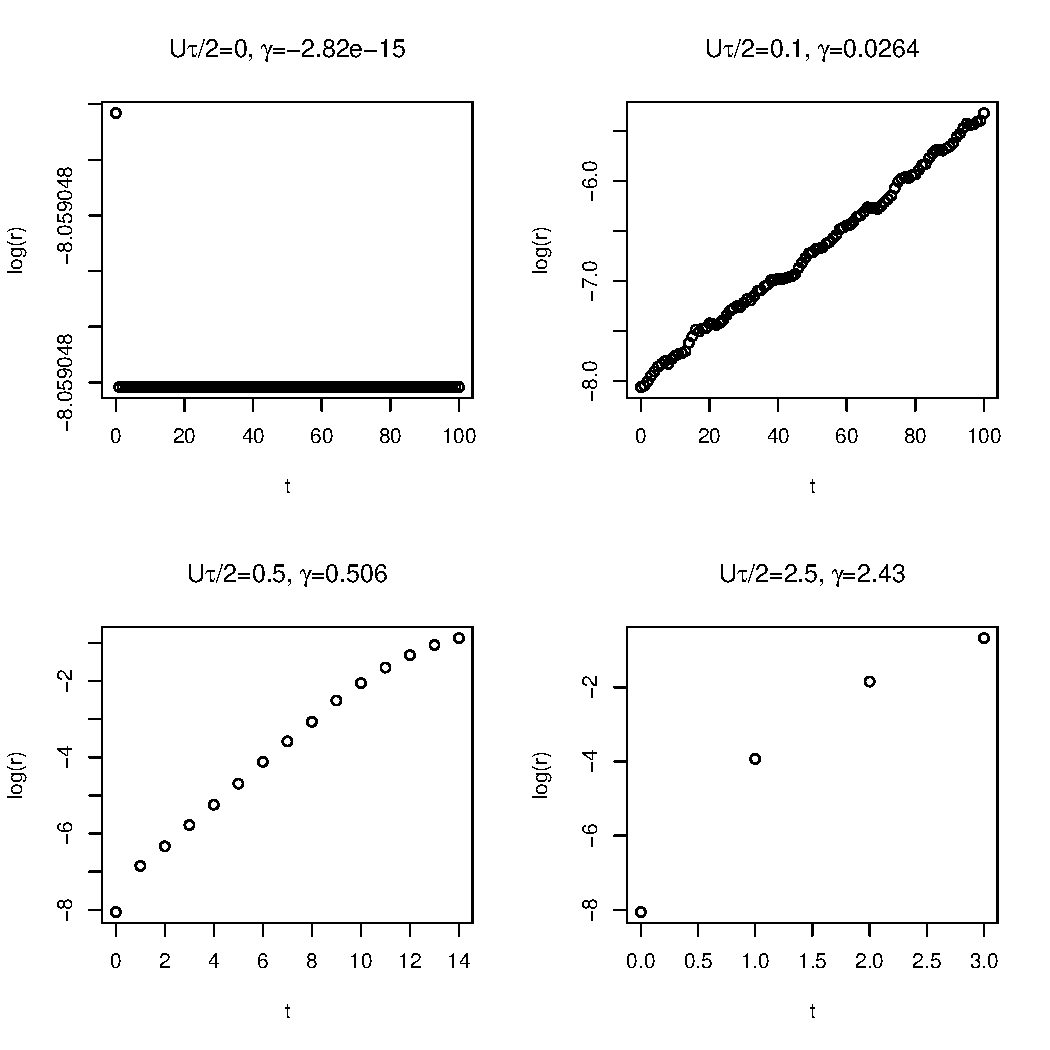
\includegraphics[width=0.95\textwidth]{../code/figure/gamma_for_different_Utot.pdf}
\par\end{centering}
\caption{Estimates of $\gamma$ for different $U\tau/2$\label{fig:gamma_Utot}}
\end{figure}

